\documentclass[11pt]{article}

\usepackage{enumerate}
\usepackage{amsmath}
\usepackage{color}
\usepackage{listings}
\usepackage{python}
\usepackage{graphicx}
\usepackage{adjustbox}

\graphicspath{{Figures/}}


\newenvironment{equ}{$\hfill\begin{aligned}[t]}{\end{aligned}\hfill \null$}

\lstset{
    tabsize=2
}

\begin{document}

\title{\vspace{-8ex}Stats 330 Assignment 10}
\author{Adam Hammes $\bullet$ hammesa@iastate.edu $\bullet$ Section B}
\maketitle


\section*{Problem 1}

\begin{enumerate}[(a)]
\item
	\begin{tabular}{ r | c | c | c}
		Set & 1 & 2 & 3 \\
		\hline
		Mean & 10.04 & 1.63 & 10.95 \\
		\hline
		Median & 10.10 & 0.98 & 10.93 \\
		\hline
		Stdev & 1.97 & 2.05 & 1.14 \\
		\hline
		1st Quartile & 8.69 & 0.50 & 10.02 \\
		\hline
		3rd Quartile & 11.36 & 1.90 & 11.87
	\end{tabular}

\item \adjustbox{valign=t} {
	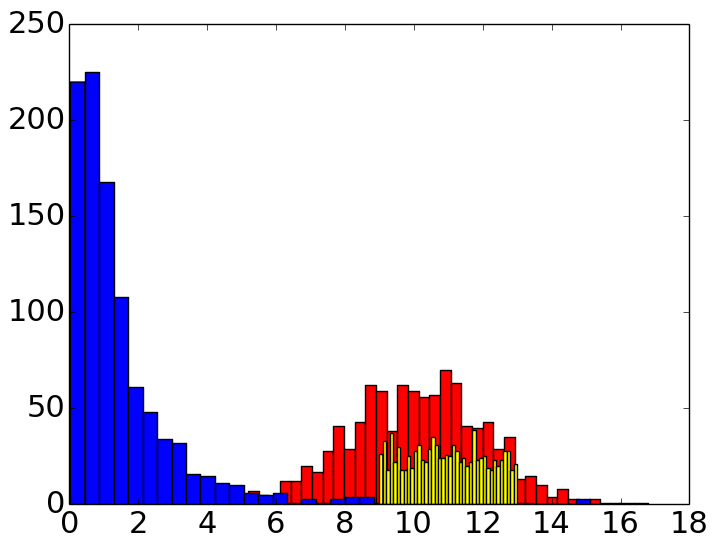
\includegraphics[scale = 0.7]{Histogram.png}
	}

\item \adjustbox{valign=t} {
	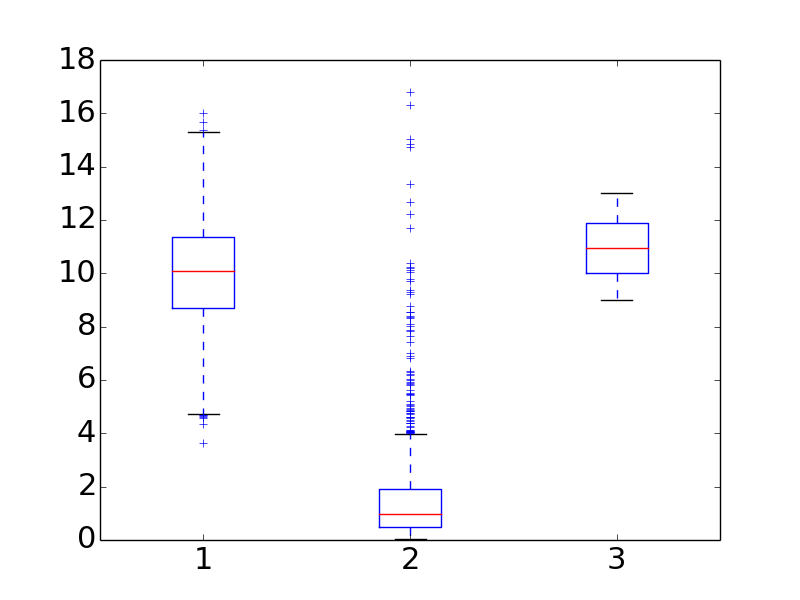
\includegraphics[scale = 0.7]{Boxplot.png}
	}


\end{enumerate}

\end{document}